%-------------------------
% Resume in Latex
% Author : Aleksei Lapin
% Based off of: https://github.com/sb2nov/resume
% License : MIT
%------------------------
\documentclass[letterpaper,11pt]{article}
\usepackage[utf8]{inputenc}
\usepackage[T2A]{fontenc}
\usepackage[russian,english]{babel}
\usepackage{latexsym}
\usepackage[empty]{fullpage}
\usepackage{titlesec}
\usepackage{marvosym}
\usepackage[usenames,dvipsnames]{color}
\usepackage{verbatim}
\usepackage{enumitem}
\usepackage[hidelinks]{hyperref}
\usepackage{fancyhdr}
\usepackage{tabularx}
\usepackage{outlines}
\usepackage{ifthen}
\usepackage{xltabular}
\usepackage{graphicx}
\usepackage{fontawesome5} % icons
\input{glyphtounicode}
\usepackage[export]{adjustbox}
\usepackage{geometry}
\geometry{
  a4paper,
  top=20mm, 
  right=20mm, 
  bottom=15mm, 
  left=20mm
}

\pagestyle{fancy}
\fancyhf{} % clear all header and footer fields
\fancyfoot{}
\renewcommand{\headrulewidth}{0pt}
\renewcommand{\footrulewidth}{0pt}

% Adjust margins
\addtolength{\oddsidemargin}{-0.5in}
\addtolength{\evensidemargin}{-0.5in}
\addtolength{\textwidth}{1in}
\addtolength{\topmargin}{-.5in}
\addtolength{\textheight}{1.0in}

\urlstyle{same}

\raggedbottom
\raggedright
\setlength{\tabcolsep}{0in}

% Sections formatting
\titleformat{\section}{
  \vspace{-4pt}\scshape\raggedright\large
}{}{0em}{}[\color{black}\titlerule \vspace{-5pt}]

% Ensure that generate pdf is machine readable/ATS parsable
\pdfgentounicode=1

%-------------------------
% Custom commands
\newcommand{\resumeItem}[2]{
  \item\small{
    \textbf{#1}{: #2 \vspace{-2pt}}
  }
}

\newcommand{\resumeItemNoBold}[1]{
  \item\small{
    {\raggedright #1 \vspace{-2pt}}
  }
}

% Just in case someone needs a heading that does not need to be in a list
\newcommand{\resumeHeading}[4]{
    \begin{tabular*}{0.99\textwidth}[t]{l@{\extracolsep{\fill}}r}
      \textbf{#1} & #2 \\
      \textit{\small#3} & \textit{\small #4} \\
    \end{tabular*}\vspace{-5pt}
}

\newcommand{\resumeSubheading}[4]{
  \vspace{-1pt}\item
    \begin{tabular*}{0.97\textwidth}[t]{p{0.7\textwidth}@{\extracolsep{\fill}}r}
      \textbf{#1} & #2 \\
      \textit{\small\raggedright#3} & \textit{\small #4} \\
    \end{tabular*}\vspace{-5pt}
}

\newcommand{\resumeSubSubheadingItem}[3]{
  \vspace{-1pt}\item
    \begin{tabular*}{0.97\textwidth}{l@{\extracolsep{\fill}}r}
      \textbf{#1} | {#2} & \textit{\small #3} \\
    \end{tabular*}\vspace{-5pt}
}


\newcommand{\resumeSubSubheading}[2]{
    \begin{tabular*}{0.97\textwidth}{l@{\extracolsep{\fill}}r}
      \textit{\small#1} & \textit{\small #2} \\
    \end{tabular*}\vspace{-5pt}
}

\newcommand{\resumeSubItem}[2]{\resumeItem{#1}{#2}\vspace{-4pt}}

\renewcommand{\labelitemii}{$\circ$}

\newcommand{\resumeSubHeadingListStart}{\begin{itemize}[leftmargin=*]}
\newcommand{\resumeSubHeadingListEnd}{\end{itemize}}
\newcommand{\resumeItemListStart}{\begin{itemize}}
\newcommand{\resumeItemListEnd}{\end{itemize}\vspace{-5pt}}

\newcommand\clink[1]{{\usefont{T1}{lmtt}{m}{n} #1 }}

% Custom commands for awards with longer descriptions
\newcommand{\resumeAwardSubheading}[4]{
  \vspace{-1pt}\item
    \begin{tabular*}{0.97\textwidth}[t]{p{0.67\textwidth}@{\extracolsep{\fill}}r}
      \textbf{#1} & #2 \\
      \textit{\small\parbox[t]{0.67\textwidth}{\raggedright #3}} & \textit{\small #4} \\
    \end{tabular*}\vspace{-5pt}
}


%-------------------------------------------
%%%%%%  CV STARTS HERE  %%%%%%%%%%%%%%%%%%%%%%%%%%%%


\begin{document}

%----------HEADING-----------------
\begin{tabularx}{\linewidth}{@{}m{0.8\textwidth} m{0.2\textwidth}@{}}
    {
    \huge{\textbf{Алексей Лапин}} \newline
    \small{
        \clink{
            \href{mailto:a.lapin03@gmail.com}{\faEnvelope~\underline{a.lapin03@gmail.com}} \textbf{ | }
            {\fontdimen2\font=0.75ex \href{tel:+79217770608}{\faPhone~\underline{+7 (921) 777-06-08}}}\textbf{ | }
            \href{https://github.com/AaLexUser}{\faGithub~\underline{github.com/AaLexUser}}
        }
        \newline
        Санкт-Петербург, Россия
    }
    } &
    {
            \hfill
            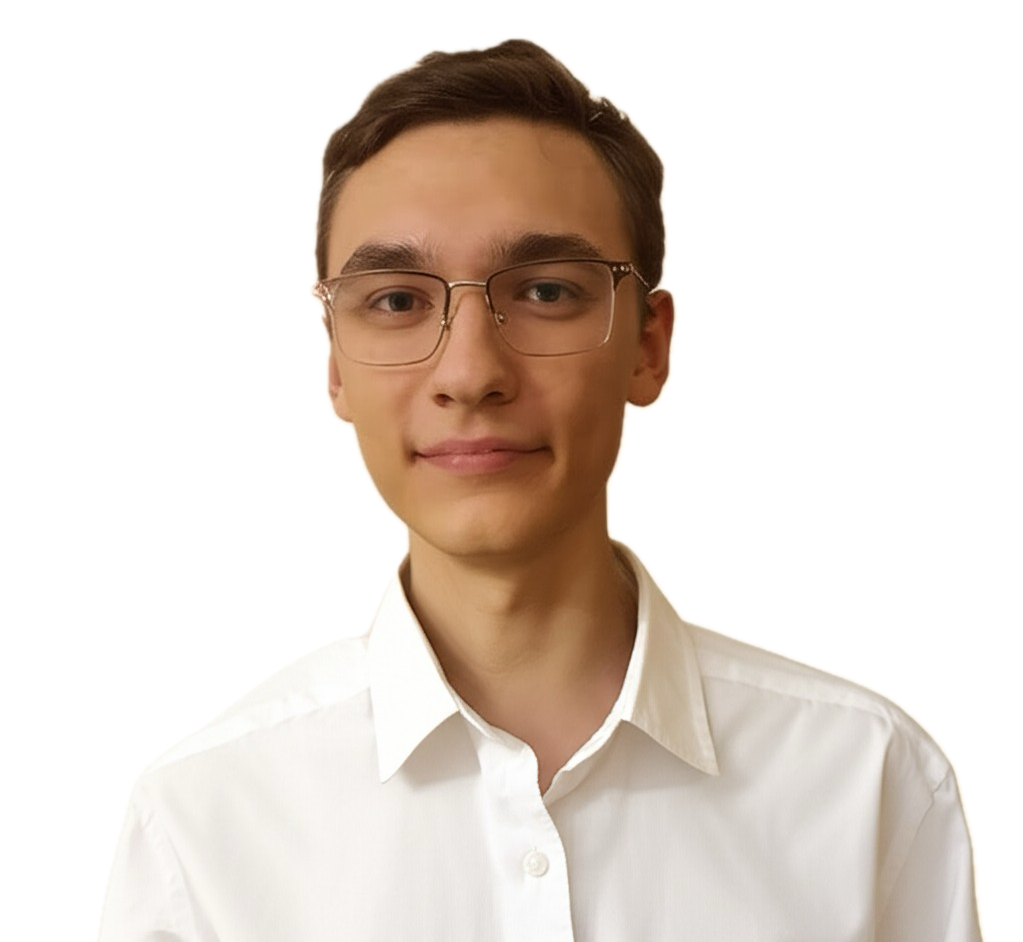
\includegraphics[width=2.8cm, frame]{./me.png}
        }
\end{tabularx}
\vspace{-25pt}

%-----------EDUCATION-----------------
\section{Образование}
\resumeSubHeadingListStart
\resumeSubheading
{\href{https://itmo.ru/}{Университет ИТМО}}{Санкт-Петербург, Россия}
{\href{https://abit.itmo.ru/program/bachelor/system_software}{Бакалавриат: Системное и прикладное программное обеспечение 09.03.04\\Средний балл: 4.42}}{Сентябрь 2021 -- Июль 2025}

\resumeSubItem{Релевантные дисциплины}{Системы искусственного интеллекта, Машинное обучение и анализ данных, Информационные системы и базы данных, Прикладная статистика, Теория вероятностей}

\resumeSubItem{Выпускная квалификационная работа}{\textbf{Разработка инструмента с открытым исходным кодом для автоматизированного машинного обучения на основе больших языковых моделей.} Разработан инструмент FEDOT.LLM — гибридная многоагентная система AutoML на основе больших языковых моделей и фреймворка FEDOT. Система объединяет БЯМ для анализа задач, предобработки признаков и генерации кода с эволюционными алгоритмами FEDOT, автоматизируя ключевые этапы ML-пайплайна и сокращая время специалиста с 2,5 часов до менее чем 1 минуты. \href{https://drive.google.com/file/d/1g1yCqSV1MXgv16vtKz-8nAQFHKlGmsp8/view?usp=sharing}{\faExternalLink*~Текст} | \href{https://drive.google.com/file/d/1eLeyHzZwujkoaeVCTZ0-hTpyyZueb1R9/view?usp=sharing}{\faExternalLink*~Краткое описание}.}
\resumeSubHeadingListEnd

%-----------JOB-----------------
\section{Опыт работы}
\resumeSubHeadingListStart
\resumeSubheading
{\href{https://aim.club/}{ИЦ ИТМО «Сильный искусственный интеллект в промышленности»}}{Санкт-Петербург, Россия}
{AI Engineer}{Июль 2024 -- настоящее время}
\resumeItemListStart
\resumeItemNoBold{Основной разработчик \textbf{мультиагентной системы} \href{https://github.com/aimclub/FEDOT.LLM}{\textbf{FEDOT.LLM}} -- \textbf{гибридная система AutoML}, позволяющая пользователям решать ML-задачи через \textbf{естественный язык}, используя БЯМ для анализа задач, предобработки признаков и генерации кода, а AutoML-FEDOT для поиска модели и оптимизации гиперпараметров.}
\resumeItemNoBold{Интегрировал FEDOT.LLM в проект коллег -- \textbf{ИИ-ассистента для химика ChemCoScientist}, проверив систему на реальных задачах.}
\resumeItemNoBold{Реализовал совместный проект \href{https://github.com/sb-ai-lab/LADS}{\textbf{LightAutoDS-Tab}} с \textbf{SberAI}, объединив наработки в области агентных систем для \textbf{FEDOT} и \textbf{LightAutoML}, что привело к написанию научной статьи.}
\resumeItemNoBold{Разработал \href{https://github.com/AaLexUser/Fedot-assistant}{\textbf{FEDOT.ASSISTANT}} — \textbf{интеллектуальный AutoML-оркестратор}, объединяющий БЯМ с фреймворками автоматизированного машинного обучения. Система автоматически анализирует задачи через CLI-интерфейс, выполняет извлечение параметров задачи с помощью БЯМ, маршрутизирует запросы между \textbf{FEDOT}, \textbf{FEDOT Industrial} и \textbf{AutoGluon} для работы с \textbf{табличными}, \textbf{временными рядами} и \textbf{мультимодальными данными}.}

\textbf{Технологии:} Python, NumPy, Pandas, Langchain, Langgraph, LiteLLM, Langfuse, Streamlit, Chromadb, FEDOT, Fedot.Industrial, Autogluon, LightAutoML.
\resumeItemListEnd
\resumeSubHeadingListEnd

\section{Награды}
\resumeSubHeadingListStart
\resumeAwardSubheading{
    \href{https://drive.google.com/file/d/1GwysoXvcKNV9y8CfY3Toe9x6AXXRlWrU/view?usp=sharing}
    {Научный Эверест}}{Санкт-Петербург, Россия}
{\textbf{Победитель ежегодного конкурса "Научный Эверест"}. Проект "Разработка инструмента с открытым исходным кодом для автоматизированного машинного обучения на основе больших языковых моделей"}{Июль 2025}
\resumeAwardSubheading{
    \href{https://drive.google.com/file/d/1w0LCMTmXbGLRT5wyzHR6HV2Q5f1fHShN/view?usp=sharing}
    {XIV Конгресс молодых ученых ИТМО}}{Санкт-Петербург, Россия}
{\textbf{Победитель номинации "Лучший доклад молодого ученого"}. Проект "Разработка open-source инструмента автоматизированного машинного обучения с использованием больших языковых моделей"}{Апрель 2025}
\resumeAwardSubheading{
    \href{https://drive.google.com/file/d/1QIoI3PejwaDDYfFeW4Al2UtjX8WS3nBv/view?usp=sharing}
    {XIV Конгресс молодых ученых ИТМО}}{Санкт-Петербург, Россия}
{\textbf{Победитель номинации "Лучший доклад молодого ученого"}. Проект "Разработка сервиса разметки данных для обучения нейронных сетей"}{Апрель 2025}
\resumeAwardSubheading{
\href{https://drive.google.com/file/d/1gs8khjhjMai1iDpcuySTskslkZBpb5XG/view?usp=sharing}
{Хакатон AI Learning Lab}~\href{https://ecom.tech}{(ecom.tech)}}{Санкт-Петербург, Россия}
{\textbf{Победитель}. \href{https://github.com/AaLexUser/Data-annotation-service}{Разработка платформы разметки данных для повышения качества обучения нейронных сетей и внедрения современных AI моделей в пользовательские сервисы Самоката, Мегамаркета и Купера.}}{Февраль 2025}
\resumeSubHeadingListEnd

\section{Публикации}
\resumeItemListStart
\resumeItemNoBold{\textbf{Lapin A.}, Hromov I., Chumakov S., Mitrovic M., Simakov D., Nikitin N., Savchenko A. \textbf{LightAutoDS-Tab: Multi-AutoML Agentic System for Tabular Data} // EMNLP 2025 System Demonstrations Submission. – 2025. – URL: \href{https://openreview.net/pdf?id=eQte3nPnyu}{https://openreview.net/pdf?id=eQte3nPnyu}}
\resumeItemNoBold{\textbf{Лапин А.А.} (науч. рук. Никитин Н.О.) \textbf{Разработка open-source инструмента автоматизированного машинного обучения с использованием больших языковых моделей} // Сборник тезисов докладов конгресса молодых ученых. Электронное издание. – СПб: Университет ИТМО, [2025]. URL: \href{https://kmu.itmo.ru/digests/article/15661}{https://kmu.itmo.ru/digests/article/15661}}
\resumeItemNoBold{Ермаков Т.С., \textbf{Лапин А.А.}, Ри А.Р. (науч. рук. Кугаевских А.В.) \textbf{Разработка сервиса разметки данных для обучения нейронных сетей} // Сборник тезисов докладов конгресса молодых ученых. Электронное издание. – СПб: Университет ИТМО, [2025]. URL: \href{https://kmu.itmo.ru/digests/article/15941}{https://kmu.itmo.ru/digests/article/15941}}
\resumeItemListEnd

\section{РИДы}
\resumeSubHeadingListStart
\resumeAwardSubheading{
    \href{https://drive.google.com/file/d/1S3svSBZkPcgO_iljlJjtp_2BLJxRLlkO/view?usp=sharing}
    {Библиотека инструментов для быстрого прототипирования систем ИИ на основе больших языковых моделей ProtoLLM.Core}}{Декабрь 2024}
{\textbf{Программа для ЭВМ} № 2024690354 от 13.12.2024. Авторы: Бухановский А.В., Никитин Н.О., Калюжная А.В., Насонов Д.А., Ковальчук М.А., Басилаев Д.И., Пискуровский М.Г., Лапин А.А., Воскресенский А.С., Каминский Ю.К., Першинов А.В., Подморин Д.О., Жидковская А.Б.}{}
\resumeAwardSubheading{
    \href{https://drive.google.com/file/d/1RXsMpZGHwlr7dLZlI-l_pmf1S2LDhuqw/view?usp=sharing}
    {Программный комплекс для решения задач автоматического машинного обучения с помощью больших языковых моделей Fedot.LLM}}{Октябрь 2024}
{\textbf{Программа для ЭВМ} № 2024683108 от 08.10.2024. Авторы: Никитин Н.О., Калюжная А.В., Лапин А.А., Лопатенко Г.В., Чумаков С.В., Соколов И.Д., Иов И.Л.}{}
\resumeSubHeadingListEnd

%-----------PROJECTS-----------------
\section{Пет-Проекты}
\resumeSubHeadingListStart

\resumeSubheading{
    \href{https://github.com/AaLexUser/Rag-chatbot}
    {RAG Chatbot}}{\textit{Июнь 2024}}{Python, LangChain, Flask, ChromaDB, Ollama}{ }
\resumeItemListStart
\resumeItemNoBold{Диалоговое ИИ-приложение с использованием \textbf{Retrieval-Augmented Generation (RAG)} для предоставления релевантной информации пользователям.}
\resumeItemNoBold{Реализовал \textbf{веб-интерфейс} на Flask с возможностью загрузки файлов и отображения источников информации}
\resumeItemNoBold{Интегрировал \textbf{ChromaDB} для векторного поиска и \textbf{LangChain} для обработки запросов к локальным LLM через \textbf{Ollama}.}
\resumeItemNoBold{Создал интерактивный UI с \textbf{JavaScript}, показывающий детальную информацию об источниках при наведении.}
\resumeItemListEnd

\resumeSubheading{
    \href{https://github.com/AaLexUser/MyitmoGPT}
    {MyItmoGPT}}{\textit{Апрель 2024}}{Python, YandexGPT, Telegram Bot}{ }
\resumeItemListStart
\resumeItemNoBold{Телеграмм бот для получения расписания с my.itmo путем естественного разговора с YandexGPT.}
\resumeItemNoBold{Создал \textbf{промты} для \textbf{YandexGPT}, которые помогают извлекать нужную информацию из диалога с пользователем. Их ответом являются \textbf{аргументы для функции} в нужном формате. Это дало возможность получать необходимую информацию из внешних источников, недоступных LLM напрямую.}
\resumeItemNoBold{Написал \textbf{промты}, которые на основе данных из внешних источников и вопроса пользователя предоставляют точный и понятный ответ на интересующий вопрос.}
\resumeItemNoBold{Реализовал команды и ежедневные напоминания в \textbf{Telegram Боте}.}
\resumeItemListEnd

\resumeSubHeadingListEnd


%--------PROGRAMMING SKILLS------------
\section{Технические навыки}
\resumeSubHeadingListStart
\resumeSubItem{Языки Программирования}{Python, Java, TypeScript, C/C++, Clojure, SQL (PostgreSQL)}
\resumeSubItem{ML/AI Фреймворки}{LightAutoML, AutoGluon, FEDOT, FEDOT.Industrial, Langchain, Langgraph, LiteLLM, Langfuse}
\resumeSubItem{Библиотеки для Данных}{Pandas, NumPy, Matplotlib, ChromaDB}
\resumeSubItem{Веб-разработка}{Streamlit, React, Spring Boot, Spring, Spring Data}
\resumeSubItem{Инструменты разработки}{Git, GitHub Actions, Gradle, Maven, Jupyter Notebook, Google Colab}
\resumeSubHeadingListEnd
\end{document}
